\documentclass{beamer}

\usepackage[russian]{babel}
\usepackage[utf8]{inputenc}
\usepackage[outputdir=cache]{minted}

\usetheme{Madrid}
\usecolortheme{dove}
\setbeamertemplate{blocks}[rounded][shadow=false]

\title[]{Приложения комплексных чисел к решению геометрических задач}
\institute[]{ФГБОУ ВО «Вятский государственный университет»}
\date{\today}
\author[ ]{Студент ПМИб-2301-52-00 Ступников Григорий Евгеньевич \and К.ф-м.н Пушкарев Игорь Александрович}

\newcommand\frametitleSpec[1]{%
\frametitle{#1}
\section{#1}%
}


% set captions with numbers
\setbeamertemplate{caption}[numbered]

\begin{document}
\begin{frame}
   \centering
\includegraphics[width=0.4\textwidth]{images/vyatsu_logo.png}\\
   \titlepage
\end{frame}
\begin{frame}
   \frametitle{План доклада}

   \tableofcontents

\end{frame}
\begin{frame}
   \frametitleSpec{Введение}
   Метод комплексных чисел -- это расширение алгебраического метода.
   \begin{enumerate}
      \item Проблема состоит в том, что для данного метода отсутствуют программные материалы для внедрения в среду самостоятельного и школьного обучения.
      \item Целью данной работы является изучение метода комплексных чисел при решении геометрических задач, реализация программной верификации решения выбранных задач. Для достижения цели необходимо выполнить следующие задачи:
            \begin{itemize}
               \item Изучить имеющиеся способы применения алгебры комплексных чисел при решении геометрических задач.
               \item Выбрать задачи, на которых будет рассматриваться практическое применение метода.
               \item Решение задач с применением метода комплексных чисел и без них
               \item Сравнение решений задач.
               \item Реализация программной верификации решения задач с применением метода.
            \end{itemize}
   \end{enumerate}
\end{frame}

\begin{frame}
   \frametitleSpec{Основы метода}
   \begin{columns}
      \begin{column}{0.5\textwidth}
         Комплексное число \(z\) -- число вида $x + iy$. У числа \(z\) можно выделить действительную $x = Re(z)$ и мнимую $y=Im(z)$ части. Каждое комплексное число представимо в виде точки на декартовой плоскости и наоборот. В таком случае точка обозначается как \(M(z)\), где \(z\) --- комплексные координаты точки \(M\).
      \end{column}
      \begin{column}{0.5\textwidth}
         \begin{figure}
            \centering
            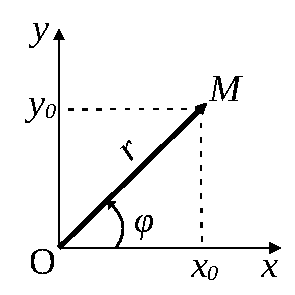
\includegraphics[width=1\textwidth]{images/theory-1.pdf}
            \caption{Изображение точки \(M(z)\) на плоскости}
            \label{img1}
         \end{figure}
      \end{column}
   \end{columns}
\end{frame}

% TASK BEGIN
\begin{frame}
   \frametitleSpec{Задачи}
   \subsection{Задача 1}
   \begin{block}{Задача 1. Постановка задачи:}
      \begin{columns}
         \begin{column}{0.5\textwidth}
            Точка \(D\) симметрична центру описанной около треугольника ABC окружности, относительно прямой AB.
            Доказать, что расстояние CD выражается формулой
            \begin{equation}
               CD^2 = R^2 +AC^2 + BC^2 - AB^2
               \label{t1:f1}
            \end{equation}
            где R - радиус описанной окружности.
         \end{column}
         \begin{column}{0.5\textwidth}
            \begin{figure}[h]
               \centering
               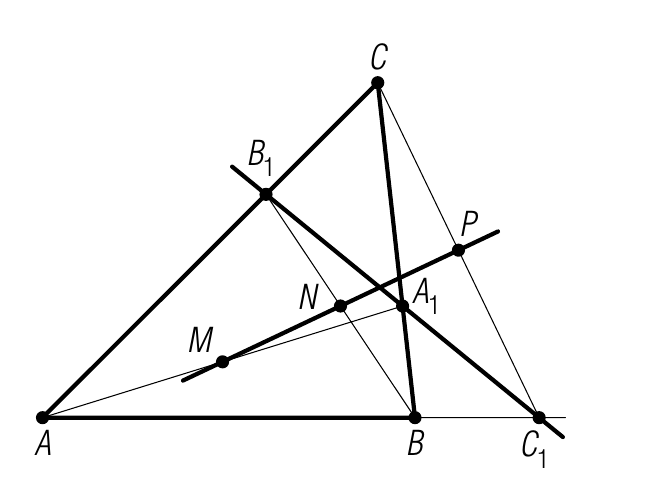
\includegraphics[width=1\textwidth]{images/task1.png}
               \caption{Иллюстрация к задаче}
               \label{t1:im}
            \end{figure}
         \end{column}
      \end{columns}
   \end{block}
\end{frame}

\begin{frame}
   \begin{block}{Задача 1. Решение задачи:}
      Т.к \(d = a + b\), то верно следующее:
      \begin{flalign*}
          & CD^2 = 3R^2 + (a\bar{b} + \bar{a}b) - (a\bar{c} +  \bar{a}c) - (b\bar{c} + \bar{b}c). &
      \end{flalign*}
      Этому же выражению равна правая часть доказываемого
      равенства:
      \begin{flalign*}
          & R^2 + AC^2 + BC^2 - AB^2 = 3R^2  + (a\bar{b} + \bar{a}b) - (a\bar{c} + \bar{a}c) - (b\bar{c} + \bar{b}c) & \\
      \end{flalign*}
      Таким образом утверждение (\ref{t1:f1}) верно, что и требовалось доказать.
   \end{block}
\end{frame}

\begin{frame}
   \begin{columns}
      \begin{column}{0.4\textwidth}
         \begin{block}{Задача 1. Вычислительная иллюстрация на частном случае:}
         \end{block}
      \end{column}
      \begin{column}{0.6\textwidth}
         \begin{figure}[h]
            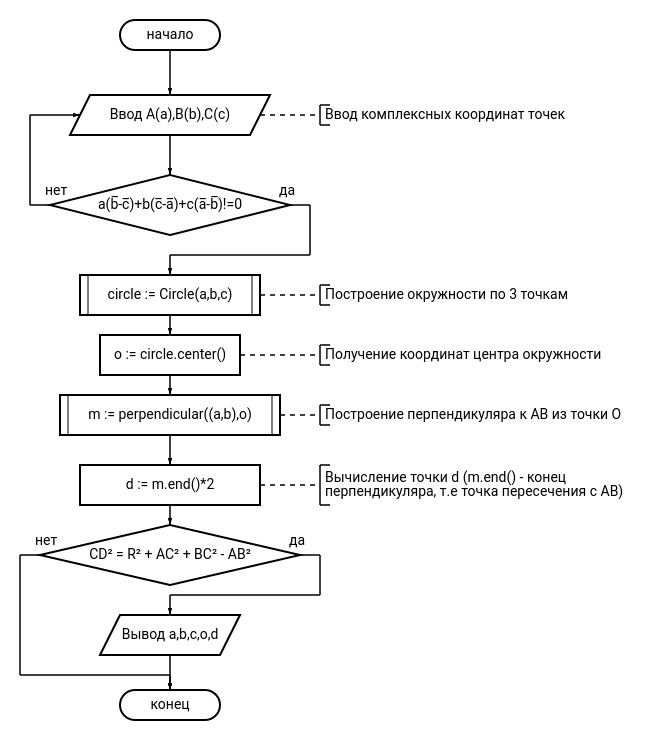
\includegraphics[width=1\textwidth]{images/task1-diagram.png}
         \end{figure}
      \end{column}
   \end{columns}
\end{frame}

\begin{frame}[fragile]
   Демонстрация работы программной реализации алгоритма:
   \begin{minted}{text}
      [codetest] ./realease.app 1
      Task #1
      Enter coordinates of triangle's points:
       A: 0 0
       B: 4 0
       C: 2 3.24
      Computed coordinates:
       A: 0 + 0i
       B: 4 + 0i
       C: 2 + 3.24i
       D: 2 + -1i
       O: 2 + 1i
      -----
   \end{minted}
\end{frame}
% TASK END

% TASK BEGIN
\begin{frame}
   \subsection{Задача 2}
   \begin{block}{Задача 2}
      Постановка задачи:
      Точка \(M\) --- середина дуги \(AB\) окружности.
      Доказать, что для произвольной точки N этой
      окружности имеет место
      равенство
      \begin{equation}
         \left\lvert AM^2-MN^2 \right\rvert = AN \cdot BN.
         \label{t2:f1}
      \end{equation}
      Решение задачи:

      Находим:
      \(AN \cdot BN = \left\lvert a-n \right\rvert \cdot \left\lvert b-n \right\rvert
      = \left\lvert (a-n)(\bar{a}-n)\right\rvert
      = \left\lvert a\bar{a} - na - n\bar{a} + n^2 \right\rvert
      = \left\lvert 1 + n^2 - n(a+\bar{a})\right\rvert.\)
      \bigskip

      Так как \(AM^2 =(a-1)(\bar{a}-1)\) и \(MN^2 =(n-1)(\bar{n}-1)\), то
      \(\left\lvert AM^2 - MN^2 \right\rvert = \left\lvert n+\bar{n}-(a+\bar{a}) \right\rvert\).
      Умножив это равенство на \(\left\lvert n \right\rvert=1\), получим:

      \(\left\lvert AM^2 - MN^2 \right\rvert = \left\lvert n^2 +1-n(a+\bar{a})\right\rvert = AN \cdot BN\).
   \end{block}
\end{frame}

\begin{frame}
   \begin{columns}
      \begin{column}{0.3\textwidth}
         \begin{block}{Задача 2. Вычислительная иллюстрация на частном случае:}
         \end{block}
      \end{column}
      \begin{column}{0.7\textwidth}
         \begin{figure}[h]
            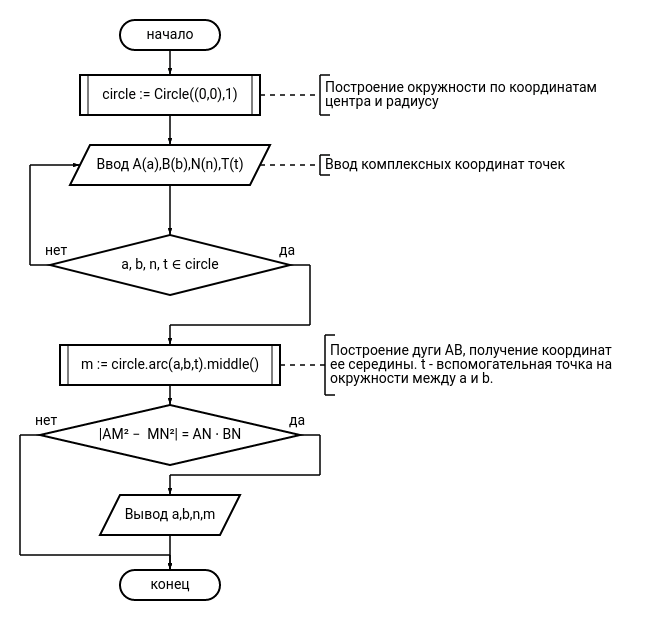
\includegraphics[width=1\textwidth]{images/task2-diagram.png}
         \end{figure}
      \end{column}
   \end{columns}
\end{frame}

\begin{frame}[fragile]
   Демонстрация работы программной реализации алгоритма:
   \begin{minted}{text}
      [codetest] ./realease.app 2
      Task #2
      Enter coordinates of a,b,n,t points (must
       conform x^2+y^2 = 1, t between a and b):
       A: 0.5 0.866
       B: 0.5 -0.866
       N: -1 0
       T: 0.707 0.707
      Computed coordinates:
       A: 0.5 + 0.87i
       B: 0.5 + -0.87i
       N: -1 + 0i
       T: 0.71 + 0.71i
       M: 1 + 0i
      -----
   \end{minted}
\end{frame}
% TASK END

% TASK BEGIN
\begin{frame}
   \subsection{Задача 3}
   \begin{block}{Задача 3. Постановка задачи:}
      \begin{columns}
         \begin{column}{0.5\textwidth}
            Докажите, что сумма квадратов диагоналей параллелограмма
            равна сумме квадратов всех его сторон (Рис. \ref{t3:im}).
            Таким образом, требуется доказать, что
            \begin{equation}
               AD^2 + BC^2 = AB^2 +CD^2 + BD^2 + AC^2
               \label{t3:f1}
            \end{equation}

         \end{column}
         \begin{column}{0.5\textwidth}
            \begin{figure}[h]
               \centering
               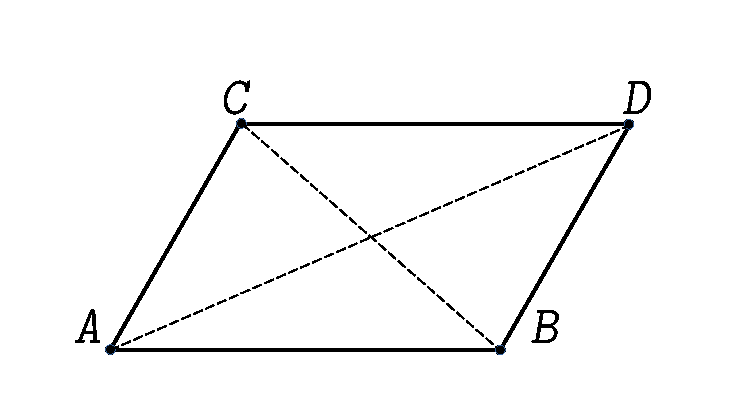
\includegraphics[width=1\textwidth]{images/task3.pdf}
               \caption{Иллюстрация к задаче}
               \label{t3:im}
            \end{figure}
         \end{column}
      \end{columns}
   \end{block}
\end{frame}

\begin{frame}
   \begin{block}{Задача 3. Решение задачи:}

      Кратко
   \end{block}
\end{frame}


\begin{frame}
   \begin{columns}
      \begin{column}{0.3\textwidth}
         \begin{block}{Задача 3. Вычислительная иллюстрация на частном случае:}
         \end{block}
      \end{column}
      \begin{column}{0.7\textwidth}
         \begin{figure}[h]
            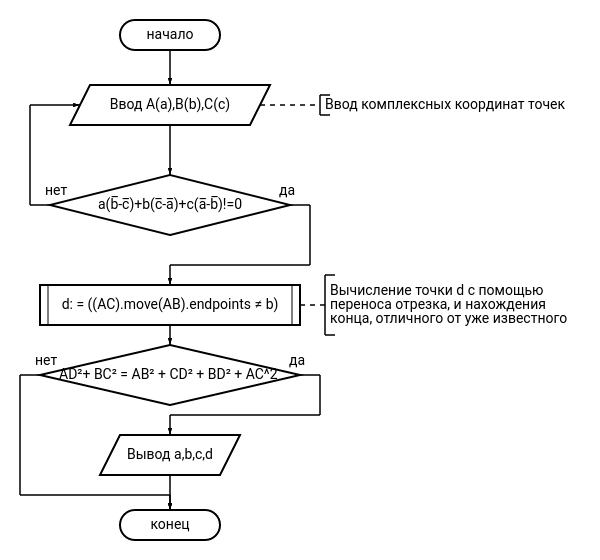
\includegraphics[width=1\textwidth]{images/task3-diagram.png}
         \end{figure}
      \end{column}
   \end{columns}
\end{frame}

\begin{frame}[fragile]
   Демонстрация работы программной реализации алгоритма:
   \begin{minted}{text}
      [codetest] ./realease.app 3
      Task #3
      Enter coordinates of triangle's points:
       A: 1 0
       B: 5 0
       C: 2 3
      Computed coordinates:
       A: 1 + 0i
       B: 5 + 0i
       C: 2 + 3i
       D: 6 + 3i
      -----
   \end{minted}
\end{frame}
% TASK END

% TASK BEGIN
\begin{frame}
   \subsection{Задача 4}
   \begin{block}{Задача 4. Постановка задачи:}


      Доказать, что если некоторая прямая пересекает прямые, содержащие стороны \(BC\), \(CA\), \(AB\) треугольника \(ABC\), в точках \(A_1\) , \(B_1\) , \(C_1\) соответственно, то середины отрезков \(AA_1\) , \(BB_1\) , \(CC_1\) коллинеарны.

      \begin{figure}[h]
         \centering
         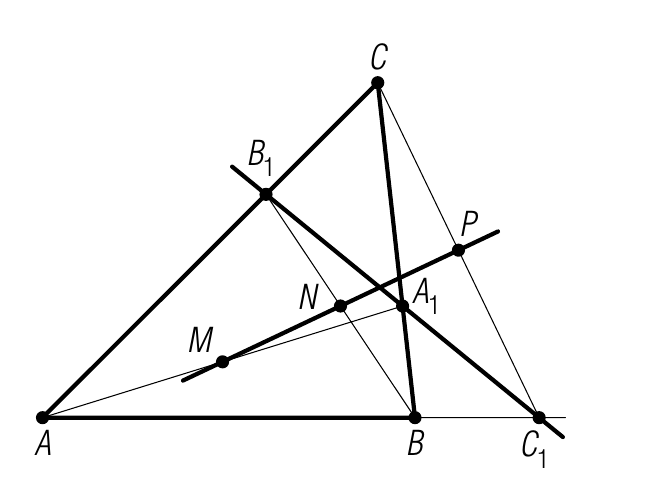
\includegraphics[width=0.4\textwidth]{images/task1.png}
         \label{task4}
      \end{figure}
   \end{block}
\end{frame}

\begin{frame}
   \begin{block}{Задача 4. Решение задачи:}

      Кратко
   \end{block}
\end{frame}

\begin{frame}
   \begin{columns}
      \begin{column}{0.3\textwidth}
         \begin{block}{Задача 4. Вычислительная иллюстрация на частном случае:}
         \end{block}
      \end{column}
      \begin{column}{0.7\textwidth}
         \begin{figure}[h]
            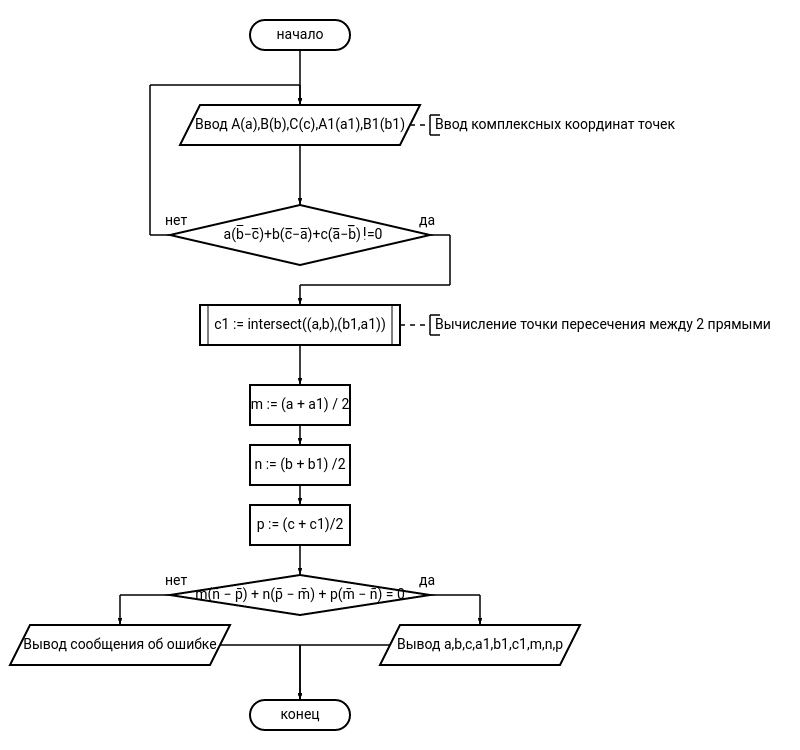
\includegraphics[width=1\textwidth]{images/task4-diagram.png}
         \end{figure}
      \end{column}
   \end{columns}
\end{frame}

\begin{frame}[fragile]
   Демонстрация работы программной реализации алгоритма:
   \begin{minted}{text}
      [codetest] ./realease.app 4
      Task #4
      Enter coordinates of a,b,c,a1,b1 points:
       A: 0 0
       B: 10 0
       C: 8 10
       A1: 9.5 2.5
       B1: 4 5
      Computed coordinates:
       A: 0 + 0i
       B: 10 + 0i
       C: 8 + 10i
       A1: 9.5 + 2.5i
       B1: 4 + 5i
       C1: 15 + 0i
       M: 4.75 + 1.25i
       N: 7 + 2.5i
       P: 11.5 + 5i
   \end{minted}
\end{frame}
% TASK END

% TASK BEGIN
\begin{frame}
   \subsection{Задача 5}
   \begin{block}{Задача 5. Постановка задачи:}


      Доказать, что если некоторая прямая пересекает прямые, содержащие стороны \(BC\), \(CA\), \(AB\) треугольника \(ABC\), в точках \(A_1\) , \(B_1\) , \(C_1\) соответственно, то середины отрезков \(AA_1\) , \(BB_1\) , \(CC_1\) коллинеарны.

      \begin{figure}[h]
         \centering
         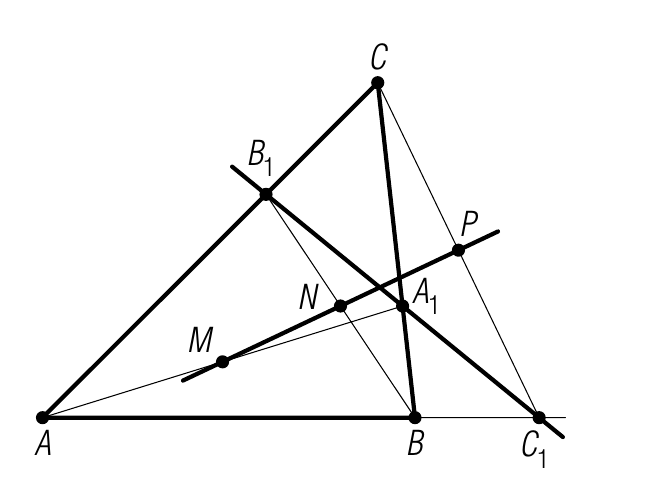
\includegraphics[width=0.4\textwidth]{images/task1.png}
         \label{task5}
      \end{figure}
   \end{block}
\end{frame}

\begin{frame}
   \begin{block}{Задача 5. Решение задачи:}

      Кратко
   \end{block}
\end{frame}

\begin{frame}
   \begin{columns}
      \begin{column}{0.3\textwidth}
         \begin{block}{Задача 5. Вычислительная иллюстрация на частном случае:}
         \end{block}
      \end{column}
      \begin{column}{0.7\textwidth}
         \begin{figure}[h]
            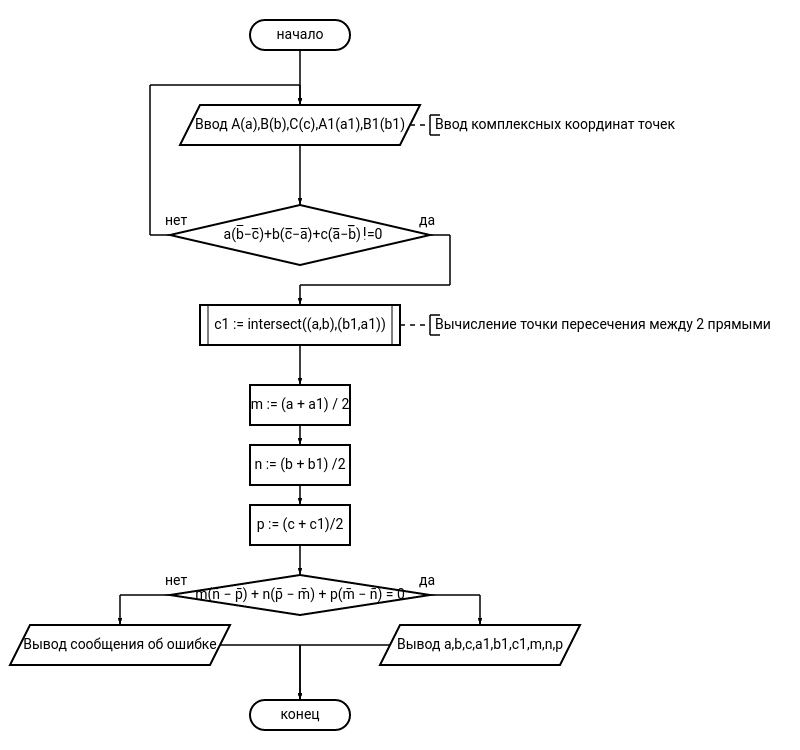
\includegraphics[width=1\textwidth]{images/task5-diagram.png}
         \end{figure}
      \end{column}
   \end{columns}
\end{frame}

\begin{frame}[fragile]
   Демонстрация работы программной реализации алгоритма:
   \begin{minted}{text}
      [codetest] ./realease.app 5
      Task #5
      Enter coordinates of a,b,c,d points (must be
       points of quadrilateral):
       A: 0 -1
       B: 2 -1
       C: 0 1
       D: 2 1
      Computed coordinates:
       A: 0 + -1i
       B: 2 + -1i
       C: 0 + 1i
       D: 2 + 1i
       O: 1 + 0i
      -----
   \end{minted}
\end{frame}
% TASK END

% TASK BEGIN
\begin{frame}
   \subsection{Задача 6}
   \begin{block}{Задача 6. Постановка задачи:}


      Доказать, что если некоторая прямая пересекает прямые, содержащие стороны \(BC\), \(CA\), \(AB\) треугольника \(ABC\), в точках \(A_1\) , \(B_1\) , \(C_1\) соответственно, то середины отрезков \(AA_1\) , \(BB_1\) , \(CC_1\) коллинеарны.

      \begin{figure}[h]
         \centering
         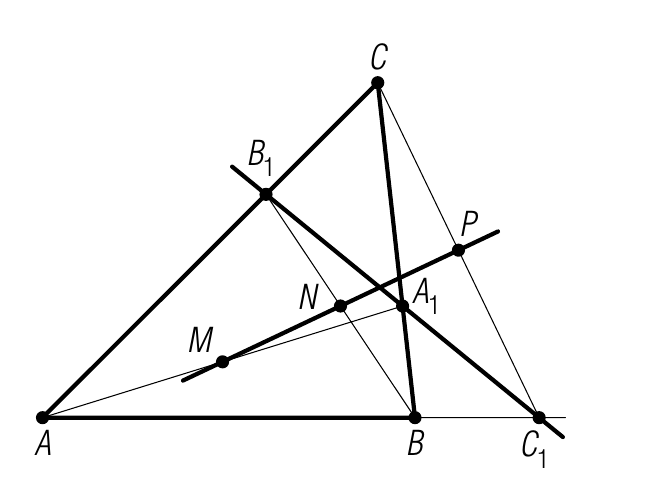
\includegraphics[width=0.4\textwidth]{images/task1.png}
         \label{task6}
      \end{figure}
   \end{block}
\end{frame}

\begin{frame}
   \begin{block}{Задача 6. Решение задачи:}
      Кратко
   \end{block}
\end{frame}

\begin{frame}
   \begin{columns}
      \begin{column}{0.3\textwidth}
         \begin{block}{Задача 6. Вычислительная иллюстрация на частном случае:}
         \end{block}
      \end{column}
      \begin{column}{0.6\textwidth}
         \begin{figure}[h]
            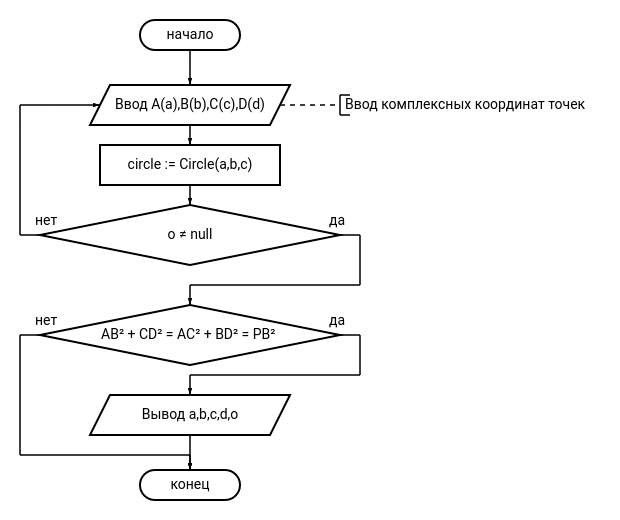
\includegraphics[width=1\textwidth]{images/task6-diagram.png}
         \end{figure}
      \end{column}
   \end{columns}
\end{frame}

\begin{frame}[fragile]
   Демонстрация работы программной реализации алгоритма:
   \begin{minted}{text}
      [codetest] ./realease.app 6
      Task #6
      Enter coordinates of a,b,c,d points (must be 
       points of quadrilateral):
       A: 1 0
       B: 3 0
       C: 1 2
       D: 3 2
      Computed coordinates:
       A: 1 + 0i
       B: 3 + 0i
       C: 1 + 2i
       D: 3 + 2i
       O: 2 + 1i
       P1: 1 + 1i
       P2: 3 + 1i
       T1: 2 + 0i
       T2: 2 + 2i
   \end{minted}
\end{frame}
% TASK END

\begin{frame}
   \frametitleSpec{О программной реализации задач}
   Решение всех задач написано на языке C++ в виде части программы для решения задач из данной работы.
   Программа (содержащая решение всех задач) поддерживает следующие функции (кроме решения задач):
   \begin{itemize}
      \item запуск нескольких задач из командной строки
      \item вывод информации в виде, пригодном для обработки сторонними программами.
   \end{itemize}
   Кроме того, для тестирования программы написана программа тестирования и тесты к ней.
   \begin{figure}[h]
      \centering
      
\includegraphics[width=0.25\textwidth]{images/cpp-logo.png}
   \end{figure}
\end{frame}
\begin{frame}
   \frametitleSpec{Заключение}

\end{frame}
\begin{frame}
   \begin{center}
      {\huge Спасибо за внимание!}
   \end{center}
\end{frame}
\end{document}
